\section{Open and Closed Sets} 

  The first thing to define is a topology. 

  \begin{definition}[Topology]
    Let $X$ be a set and $\T$ be a family of subsets of $X$. Then $\T$ is a \textbf{topology} on $X$\footnote{I will use script letters to denote topologies and capital letters to denote sets.} if it satisfies the following properties. 
    \begin{enumerate}
      \item \textit{Contains Empty and Whole Set}: 
      \begin{equation}
        \emptyset, X \in \T
      \end{equation}

      \item \textit{Closure Under Union}. If $\{U_\alpha\}_{\alpha \in A}$ is a class of sets in $\T$, then 
      \begin{equation}
        \bigcup_{\alpha \in A} U_\alpha \in \T
      \end{equation}

      \item \textit{Closure Under Finite Intersection}: If $U_1, \ldots, U_n$ is a finite class\footnote{Note that we restrict property 3 to be a \textit{finite} intersection because it turns out that the finiteness of intersection allows us to prove many nice properties about topologies, which we will mention later. Another reason is that if we remove this finite restriction, the open ball topology on $\mathbb{R}$ would imply that $\cap_{i = 1}^{\infty} ( - 1/i, +1/i ) = 0$ is an open set $\implies$ all points are open sets too, which is generally not what we want in analysis. 
      } of sets in $\T$, then 
      \begin{equation}
       \bigcap_{i=1}^{n} U_i \in \T
      \end{equation}
    \end{enumerate}
    A \textbf{topological space} is denoted $(X, \T)$. 
  \end{definition}

  This leads to the most general definition of an open set. Note that an open set doesn't really mean anything without talking about with respect to its topology. 

  \begin{definition}[Open Set]
    The elements of $\T$ are called \textbf{open sets} in $X$.\footnote{As implied from the definition of a topology, the arbitrary union and finite intersection of any number of open sets is an open set.} 
    \begin{enumerate}
      \item An open set $U$ which contains a point $x$ is called an \textbf{open neighborhood} of $x$, denoted $U_x$. 
      \item Given an open neighborhood $U_x$ of $x$, the set $U_x \setminus \{x\}$ is called the \textbf{punctured open neighborhood} of $x$. 
    \end{enumerate}
  \end{definition}

  For the sake of giving at least one nontrivial example, here is an example of a finite topology. 

  \begin{example}[Topologies of a Set of Cardinality 3]
    There are a total of 29 topologies that we can construct on $\{1, 2, 3\}$. Two such examples are 
    \begin{enumerate}
      \item $\{\emptyset, \{1, 2\}, \{1, 2, 3\}\}$ 
      \item $\{\emptyset, \{3\}, \{2, 3\}, \{1, 2, 3\}\}$
    \end{enumerate}
  \end{example} 

  When we define a new topology, we must first prove that they are topologies, and so these definitions are really theorems. However, I will introduce them as definitions and reserve the theorem environment for actual theorems. 

  \begin{definition}[Discrete, Indiscrete Topologies]
    Given a set $X$, 
    \begin{enumerate}
      \item $2^X$ is a topology, called the \textbf{discrete topology}. 
      \item $\{\emptyset, X \}$ is a topology, called the \textbf{indiscrete topology}. 
    \end{enumerate}
  \end{definition}
  \begin{proof}
    Listed. 
    \begin{enumerate}
      \item The first property is trivially proven. From the theorems of set theory, $U_\alpha \subset X \implies \cup U_\alpha \subset X \implies \cup U_\alpha \in 2^X$. Finally the same logic holds for intersection as well. 
      \item The first property is trivially proven. We can check for the 4 combinations of unions and intersections and see that they all result in either $\emptyset$ or $X$. 
    \end{enumerate}
  \end{proof}

  \begin{definition}[Finer, Coarser Topologies]
    Suppose that $\T$ and $\T^\prime$ are two topologies on a given set $X$. If $\T \subset \T^\prime$, we say that $\T^\prime$ is \textbf{finer} than $\T$, or equivalently, we say that $\T$ is \textbf{coarser} than $\T^\prime$. 
  \end{definition}

  We can think of the topology of a set $X$ as a truck full of gravel as the open sets. If the gravel is smashed into smaller, finer pieces, then the amount of stuff that we can make from the finer gravel increases, which corresponds to a bigger topology. Clearly, the indiscrete topology is the coarsest topology and the discrete topology is the finest. 

  \begin{theorem}[Intersection of Topologies]
    Given a family of topologies $\{\T\}_{\alpha \in A}$, the set 
    \begin{equation}
      \T = \bigcap_{\alpha \in A} \T_\alpha
    \end{equation}
    is a topology. 
  \end{theorem}

  \begin{corollary}[Unique Coarsest and Finest Topology]
    Given a family of topologies $\{\T\}_{\alpha \in A}$, there exists 
    \begin{enumerate}
      \item a unique smallest topology on $X$ containing all the collections $\T_\alpha$. 
      \item a unique largest topology on $X$ contained in each $\T_\alpha$. 
    \end{enumerate}
  \end{corollary} 

  \begin{example}
    Let $X = \{a, b, c\}$, and let 
    \begin{align}
      \T_1 & = \{\emptyset, X, \{a\}, \{a, b\}\} \\
      \T_2 & = \{\emptyset, X, \{a\}, \{b, c\}\}
    \end{align}
    We claim that the 
    \begin{enumerate}
      \item smallest topology containing $\T_1, \T_2$ is 
      \begin{equation}
        \T_{1 \cup 2} = \{\emptyset, X \{a\}, \{b\}, \{a, b\}, \{b, c\}\}
      \end{equation} 
      Note that this is not simply the union of topologies. The union wouldn't have $\{b\}$, making it not a topology. 

      \item largest topology contained in $\T_1, \T_2$ is 
      \begin{equation}
        \T_{1 \cap 2} = \{\emptyset, X, \{a\}\}
      \end{equation}
      Note that this is simply the intersection of the two topologies. 
    \end{enumerate}
  \end{example}

\subsection{Basis} 

  So far so good. We have introduced a topology as a collection satisfying some properties, but given a topology on $X$, it is often a bit difficult to see whether an arbitrary set $S \subset X$ is open. For this, we have the following. 

  \begin{lemma}[A Set Full of Open Sets is Open]
    Given $X$ with a topology $\T$, let $S \subset X$. Then $S$ is open if for every $x \in S$, there exists an open neighborhood $U_x$ satisfying $x \in U_x \subset S$. 
  \end{lemma}
  \begin{proof}
    Since we can set 
    \begin{equation}
      S = \bigcup_{x \in S} U_x
    \end{equation}
    it is an arbitrary union of open sets and therefore must be open. 
  \end{proof}

  We want to continue analyzing the properties of a topology, but sometimes working with the entire topology is a bit thorny. There is a tamer representation of a topology, which can also give us the starting point to \textit{construct} topologies. 

  \begin{definition}[Basis]
    If $X$ is a set, a \textbf{basis} on $X$ is a collection $\B$ of subsets of $X$ (called \textbf{basis elements}) such that
    \begin{enumerate}
      \item For each $x \in X$, there is at least one basis element $B \in \B$ containing $x$. That is, the elements of $\B$ covers $X$. 
      \item If $x$ belongs to the intersection of two basis elements $B_1$ and $B_2$, then there is a basis element $B_3$ containing $x$ such that $B_3 \subset (B_1 \cap B_2)$. 
    \end{enumerate}
  \end{definition} 

  The name gives away the clue that a topology may be created from this basis.  

  \begin{theorem}[Basis to Topology]
    Given a basis $\B$ on a set $X$, we can define a topology $\T$, called the \textbf{topology generated by $\B$}, in the following equivalent ways. 
    \begin{enumerate}
      \item $\T$ consists of subsets $U$ of $X$ satisfying the property that for each $x \in U$, there exists a basis element $B \in \B$ such that $x \in B \subset U$.\footnote{Note that since we can always set $U = \emptyset$, the basis doesn't need to contain $\emptyset$. }
      \begin{center}
        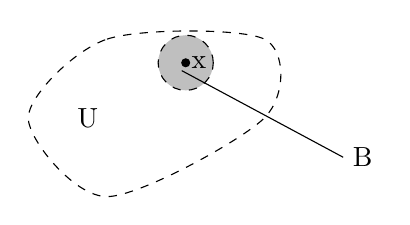
\begin{tikzpicture}
        \draw[dashed] plot [smooth cycle] coordinates {(0,0) (1,1) (3,1) (3,0) (1,-1)};
        \node [right] at (0.5,0) {U};
        \draw[fill=lightgray,dashed] (2,0.7) circle [radius=0.35];
        \draw[fill] (2, 0.7) circle [radius=0.05];
        \node [right] at (1.95,0.7) {x};
        \node [right] at (4,-0.5) {B};
        \draw (1.95,0.6)--(4,-0.5);
        \end{tikzpicture}
      \end{center}

      \item $\T$ consists of all possible unions of elements in $\B$. 
      \begin{equation}
        \T \equiv \Big\{ \bigcup_i B_i \mid B_i \in \B\Big\}
      \end{equation}
    \end{enumerate}
  \end{theorem} 
  \begin{proof}
    We prove that the 2 methods generate a topology, and then finally prove that it they are the same topology. 
    \begin{enumerate}
      \item Clearly, $\emptyset$ and $X$ itself are in $\T$. To prove property 2, given a certain indexed family of subsets $\{U_\alpha\}_{\alpha \in I}$ of $\T$, we must show that 
      \begin{equation}
        U = \bigcup_{\alpha \in I} U_\alpha \in \T
      \end{equation}
      Given $x \in U$, there exists at least one index $\alpha$ such that $x \in U_\alpha$. Since $U_\alpha \in \T$ already, there exists a basis element $b \in \B$ such that $x \in b \subset U_\alpha$. But 
      \begin{equation}
        U_\alpha \subseteq U \implies b \subset U
      \end{equation}
      So, by definition, any arbitrary union of $U$ of these subsets is also in $\T$. 

      To prove property 3, we must show that 
      \begin{equation}
        W = \bigcap_{\alpha \in I} U_\alpha \in \T
      \end{equation}
      Given $x \in W$, by definition of a basis element, there exists a $b \in \B$ such that 
      \begin{equation}
        x \in b \subset (U_\beta \cap U_\gamma) \forall \beta, \gamma \in I \implies \text{ there exists } \Tilde{b} \in \B \text{ s.t. } x \in \Tilde{b} \subset \bigcap_{\alpha \in I} U_\alpha
      \end{equation}
      By definition, $W$ is also open. Since this arbitrary set of subsets $\T$ suffices the 3 properties, it is a topology of $X$ by definition. 

      \item $(\rightarrow)$ Given a collection of elements in $\B$, they are also elements of $\T$. Since $\T$ is a topology, their union in also in $\T$. 

      $(\leftarrow)$ Given an open set $U \in \T$, for every point $x \in U$, by definition we can choose a basis element $b \in \B$ such that $x \in b \subset U$. Then, the union of all these basis elements is by definition $b$. 
        
    \end{enumerate}
  \end{proof}

  We have learned how to go from a basis to a topology. The following lemma tells us how to identify a basis within a topology. 

  \begin{theorem}[Topology to Basis]
    Let $(X, \T)$ be a topological space, and let $\B$ be a collection of open subsets of $X$ such that for every open set $U$ and each $x \in U$, there exists an element $B \in \B$ such that
    \begin{equation}
      x \in B \subset U
    \end{equation}
    Then, $\B$ is a basis for the topology of $X$. 
  \end{theorem}
  \begin{proof}
    Note that there are two claims here: $\B$ is a basis and the topology that $\B$ generates is equal to $\T$. 
    \begin{enumerate}
      \item To prove that $\B$ is a basis, note that $X$ is an open set, and by assumption, for every $x \in X$, there exists a $B \in \B$ s.t. $x \in B \subset X$. Therefore $\B$ covers $X$. Now take two basis elements $B_1, B_2 \in \B$ with $x \in B_1 \cap B_2$. Since we know that $B_1, B_2$ are open, $B_1 \cap B_2$ is open and so for each $x \in B_1 \cap B_2$, there exists a basis element $B_3$ s.t. $x \in B_3 \in (B_1 \cap B_2)$. Thus $\B$ is a basis. 

      \item Let us call $\T^\prime$ the topology generated by $\B$. Then, given $U \in \T$, by assumption for any $x \in U$, there exists a basis element $B \in \B$ s.t. $x \in B \subset U$, so $x \in \T^\prime$. Conversely, if $U \in \T^\prime$, then $U$ is an arbitrary union of elements $B \in \B$ where each $B$ is open in $\T$, so $U \in \T$. So $\T = \T^\prime$. 
    \end{enumerate}
  \end{proof} 

  Characterizing topologies in terms of basis is quite effective since we can work with more manageable sets. 

  \begin{lemma}[Fineness w.r.t. Basis]
    Given two topologies $\T$ and $\T^\prime$ with their bases $\B$ and $\B^\prime$, respectively, the following are equivalent. 
    \begin{enumerate}
      \item $\T^\prime$ is finer than $\T$. 
      \item For each $x \in X$ and basis element $B \in \B$ containing $x$, there exists a basis element $B^\prime \in \B^\prime$ such that $x \in B^\prime \subset B$. 
    \end{enumerate}
  \end{lemma}

  So we have seen how we can take a collection of sets satisfying the basis properties and construct a topology as the union of the sets in this collection. What happens if we can relax some of these conditions? Note that the first condition was that the basis elements must cover $X$. This is non-negotiable. However, if we remove the second requirement that a basis element must be contained in an intersection of basis elements, we can get a \textit{subbasis}. 

  \begin{definition}[Subbasis]
    A \textbf{subbasis} $\mathscr{S}$ for a topology on $X$ is a collection of subsets of $X$ whose union is equal to $X$. 
  \end{definition}

  \begin{theorem}[Subbasis to Topology]
    Given a subbasis $\mathscr{S}$ on a set $X$, the \textbf{topology generated by $\mathscr{S}$} is defined to be the collection $\T$ of all unions of finite intersections of elements of $\mathscr{S}$. 
  \end{theorem}
  \begin{proof}
    It suffices to show that the collection of finite intersections of elements form a basis. 
  \end{proof}
 
\subsection{Limit Points and Closed Sets} 

  First, we need to learn what it generally means for a point to be infinitesimally close to a set. 

  \begin{definition}[Limit Point]
    Given a topological space $(X, \T)$, let $x \in X$ be a point and $S \subset X$ a subset. $x$ is a \textbf{limit point of $S$} if every punctured neighborhood of $x$ intersects $S$.\footnote{Note that limit point are generally used to talk about points that are infinitesimally close to a set $S$. A limit point may not necessarily be in $S$, and a point of $S$ may not necessarily be a limit point. This is why we use a punctured neighborhood, rather than an open neighborhood. For continuity as we will see later, we just talk about neighborhoods since we also claim that the limit exists and the function value is the limit.} The set of all limit points of a set $S$ is denoted $S^\prime$.  
  \end{definition} 

  \begin{example}[Examples of Limit Points]
    What about the limit points that are not in $S$? Generally, there are two instances. 
    \begin{enumerate}
      \item Let $S$ represent the gray area. $B$ is in the ``interior'' of $S$ and therefore is a limit point. $A$ and $C$ are on the ``boundary'' of $S$ yet not in $S$, and we can show that they are limit points as well. 
        
      \begin{figure}[H]
        \centering 
        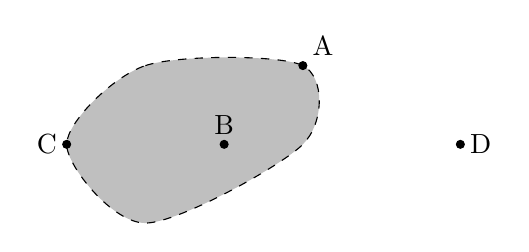
\begin{tikzpicture}
          \draw[fill=lightgray, dashed] plot [smooth cycle] coordinates {(0,0) (1,1) (3,1) (3,0) (1,-1)};
          \draw [fill] (3, 1) circle [radius=0.05];
          \node [above right] at (3,1) {A};
          \draw [fill] (2,0) circle [radius=0.05];
          \node [above] at (2,0) {B};
          \draw [fill] (0,0) circle [radius=0.05];
          \node [left] at (0,0) {C};
          \draw [fill] (5,0) circle [radius=0.05];
          \node [right] at (5, 0) {D};
        \end{tikzpicture}
        \caption{Points $A, B, C$ are limit points of the open set. }
        \label{fig:limit_boundary}
      \end{figure}

      \item A point can be at the ``convergence point'' of a sequence. 
      \begin{figure}[H]
        \centering 
        \begin{tikzpicture}
          \draw [fill] (0, 2.2) circle [radius=0.05];
          \draw [fill] (1, 2.4) circle [radius=0.05];
          \draw [fill] (2, 2) circle [radius=0.05];
          \draw [fill] (2.5, 1.8) circle [radius=0.05];
          \draw [fill] (2.6, 1.6) circle [radius=0.05];
          \draw [fill] (2.65, 1.67) circle [radius=0.05];
          \draw [fill] (2.654, 1.64) circle [radius=0.05];
          \draw [fill] (2.6543, 1.63) circle [radius=0.05];
          \node [right] at (2.6543, 1.63) {p};
        \end{tikzpicture}
        \caption{Note that if $S$ is a sequence of points in $\mathbb{R}^{2}$ that converges to $p$ without ever hitting it, we can say that $p \not\in S$ is a limit point of $S$.}
        \label{fig:limit_sequence}
      \end{figure}
    \end{enumerate}
  \end{example}

  \begin{example}[Examples of Non-Limit Points]
    There are generally two instances of non-limit points. Let $X = \mathbb{R}$ and $S = (0, 1) \cup \{2\}$. 
    \begin{enumerate}
      \item $5$ is clearly not a limit point. 
      \item $2$, although in $S$, is not a limit point since we are talking about the punctured neighborhood. A point in $S$ that is not a limit point is called an \textbf{isolated point}. 
    \end{enumerate}
  \end{example}

  \begin{definition}[Closed Set]
    A set $S \subset X$ is \textbf{closed} if its complement $X \setminus S$ is open in $\T$.\footnote{Note that open and closed sets are not mutually exclusive. A set might be open, closed, both, or neither. A set that is both open and closed is called \textbf{clopen}.}
  \end{definition}
  
  Another property, which is often used as the definition of a closed set, is that it contains all of its limit points. 

  \begin{lemma}[Closed Sets Contain Limit Points]
    A set $S \subset X$ is closed iff it contains all of its limit points. 
  \end{lemma}
  \begin{proof}
    We prove bidirectionally. 
  \end{proof}

  \begin{theorem}[Topological Space wrt Closed Sets]
    Let $X$ be a topological space. Then, the following conditions hold
    \begin{enumerate}
      \item $\emptyset$ and $X$ are clopen.
      \item Arbitrary intersections of closed sets are closed. 
      \item Finite unions of closed sets are closed. 
    \end{enumerate}
  \end{theorem}

  \begin{definition}[Dense Subsets]
    Let $S \subset (X, \tau_X)$. $S$ is \textbf{dense} in $X$ if every point $p \in X$ is a limit point of $S$. In other words, for any point $p \in X$ and any open neighborhood $U_p$ of $p$, $U_p \cap S$ is nontrivial. Otherwise, $p$ is a point of $S$. 
  \end{definition}

  The following example is a crucial fact for proving further properties of topological spaces. 

  \begin{example}
    $\mathbb{Q}^{n}$ is a dense set of $\mathbb{R}^{n}$ with the open ball topology. If we have the discrete topology of $\mathbb{R}^{2}$, an open neighborhood of a point is the point itself, so no limit points would exist beyond the points in $S$ itself. So $\mathbb{Q}^{n}$ is not dense in $\mathbb{R}^{n}$ with this topology. 
  \end{example}

\subsection{Interiors and Closures}

  Now that we've determined limit points, we would like to extend sets into their limit points. The process of doing this is called the \textit{closure} of a set. 

  \begin{definition}[Closure]
    The \textbf{closure} of set $S$ is $\overline{S}$ is defined in the following equivalent ways. 
    \begin{enumerate}
      \item $\overline{S} = S \cup S^\prime$, i.e. the union of itself and its limit points. 
      \item $\overline{S}$ is the intersection of all closed sets $C$ containing $S$. 
    \end{enumerate}
  \end{definition}
  \begin{proof}
    
  \end{proof}

  \begin{example}
    If $S$ is an open ball, $\Bar{S}$ is the closed ball. 
  \end{example}

  From semantics, it may seem like the interior and exterior (defined later) are related, but from a mathematical point of view, the interior and closure are dual notions. 

  \begin{definition}[Interior]
    Let $S \subset X$. Then, the following definitions of the \textbf{interior} of $S$, denoted $S^\circ$, are equivalent. 
    \begin{enumerate}
      \item $x \in S^\circ$ if $\exists U_x \ni x$ s.t. $U_x \subset S$. 
      \item $S^\circ$ is the union of all open sets contained in $S$. 
      \item $S^{o}$ is the complement of the closure of the complement of S. 
      \begin{equation}
        S^{o} = \big(\overline{S^{c}}\big)^{c}
      \end{equation}
    \end{enumerate}
  \end{definition}
  \begin{proof}
    
  \end{proof}

  \begin{lemma}[Open and Closed in Terms of Interiors and Closures]
    Let $S$ be a subset of some topological space $X$. 
    \begin{enumerate}
      \item $S$ is open iff $S = S^{o}$. $S^{o}$ is always open.
      \item $S$ is closed iff $S = \overline{S}$. $\overline{S}$ is always closed. 
    \end{enumerate}
  \end{lemma}

  \begin{theorem}[Clopen sets in Reals]
    There are no proper clopen sets in $\mathbb{R}$. 
  \end{theorem}

\subsection{Exteriors and Boundaries}

  \begin{definition}[Exteriors]
    Let $S \subset X$. The \textbf{exterior} of $S$, denoted $S^e$, is defined in the following equivalent ways.\footnote{We can informally think of the exterior being strictly outside of $S$ and its boundary.}
    \begin{enumerate}
      \item $S^e$ is the complement of the closure of $S$. 
      \item $S^e$ is the interior of the complement of $S$. 
    \end{enumerate}
  \end{definition}
  \begin{proof}
    
  \end{proof}

  \begin{definition}[Boundary]
    Let $S \subset X$. The \textbf{boundary} of $S$, denoted $\partial S$, is defined in the following equivalent ways. 
    \begin{enumerate}
      \item $\partial S$ is the closure minus the interior of $S$ in $X$. 
      \item $\partial S$ is the intersection of the closure of $S$ with the closure of its complement, i.e the set of all points $x$ such that every neighborhood $U_x$ intersects both the interior and exterior. 
      \item $\partial S$ is the set of points that are neither in the exterior nor the interior. 
      \item $x \in \partial S$ if every neighborhood of $x$ intersects both the interior and exterior of $S$. 
    \end{enumerate}
  \end{definition}
  \begin{proof}
    
  \end{proof}

  From the above, we get the intuitive notion that these three parts divide up the whole space. 

  \begin{theorem}[Partitioning of Space]
    Given $S \subset X$, $X$ is partitioned into the interior, boundary, and exterior of $S$. 
    \begin{equation}
      X = S^\circ \sqcup \partial S \sqcup S^e
    \end{equation}
  \end{theorem}
  \begin{proof}
    The fact that 
  \end{proof}

  One counterintuitive result is the \href{https://en.wikipedia.org/wiki/Lakes_of_Wada}{Lakes of Wada}, which are three disjoint connected open sets of the open unit square $(0, 1)^2$ with the property that they \textit{all} have the same boundary. In other words, for any point selected on the boundary of one of the lakes, the other two lakes' boundaries also contain that point. 

\subsection{Exercises} 

  \begin{exercise}[Munkres 13.1]
    Let $X$ be a topological space; let $A$ be a subset of $X$. Suppose that for each $x \in A$ there is an open set $U$ containing $x$ such that $U \subset A$. Show that $A$ is open in $X$.
  \end{exercise}
  \begin{solution}[Munkres 13.1]
    Given a $x \in A$, let us label its open neighborhood as $U_x \subset A$. We claim that 
    \begin{equation}
      A = \bigcup_{x \in A} U_x
    \end{equation} 
    We prove bidirectionally. 
    \begin{enumerate}
      \item $A \subset \cup_{x \in A} U_x$. Let $y \in A$. Then there exists an open $U_y$ containing $y$. Since $U_y$ is in the union by construction. 
      \begin{equation}
        y \in U_y \subset \bigcup_{x \in A} U_x
      \end{equation}
      \item $\cup_{x \in A} U_x \subset A$. Let $y \in \cup_{x \in A} U_x$. Then there must be some $U_y$ in this union s.t. $y \in U_y$. But by construction $U_y \subset A$, so $y \in A$. 
    \end{enumerate}
    We are done. 
  \end{solution}

  \begin{exercise}[Munkres 13.2]
    Consider the nine topologies on the set $X = \{a, b, c\}$ indicated in Example 1 of \S12. Compare them; that is, for each pair of topologies, determine whether they are comparable, and if so, which is the finer.
  \end{exercise}
  \begin{solution}[Munkres 13.2] 
    Given the figure, we denote $\tau_{i, j}$ as the topology in the $i$th row (from top) and $j$th column (from left) in the figure below. When I say for all $i, j$, I mean for all $i, j \in \{1, 2, 3\}$. 
    \begin{figure}[H]
      \centering 
      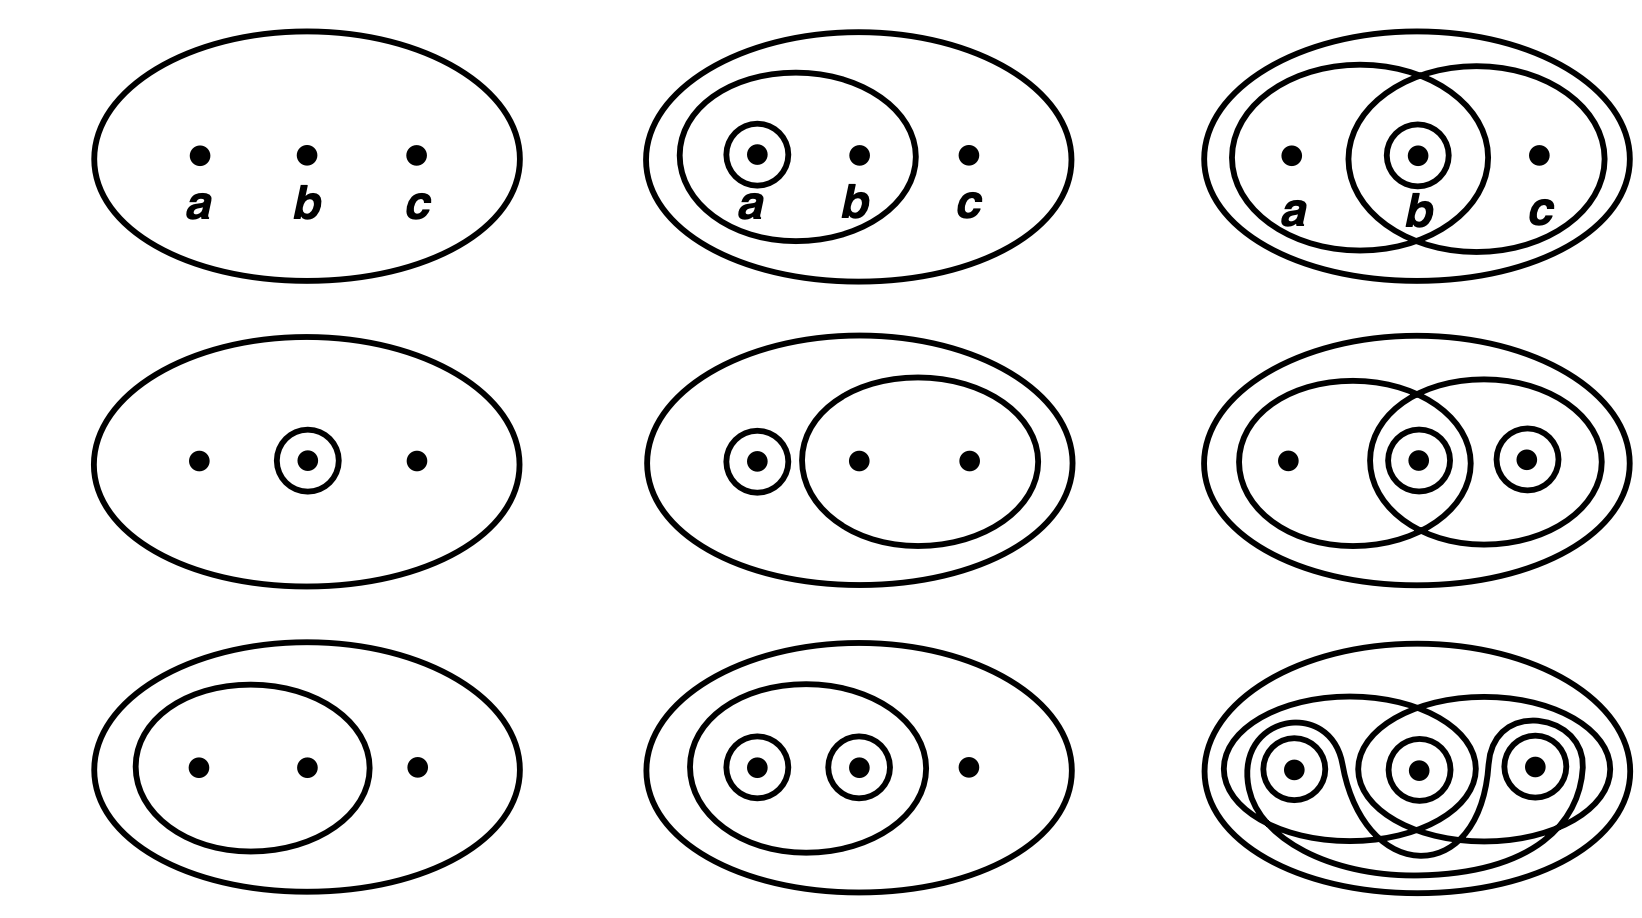
\includegraphics[scale=0.3]{img/top.png}
      \caption{} 
      \label{fig:top}
    \end{figure} 
    $\tau_{11}$ is the indiscrete topology so $\tau_{11} \subset \tau_{i, j}$ for all $i, j$, i.e. it is coarsest. $\tau_{33}$ is the discrete topology so $\tau_{i, j} \subset \tau_{3, 3}$ for all $i, j$, i.e. it is the finest. We list all other comparable topologies below. 
    \begin{enumerate}
      \item $\tau_{1, 2} \subset \tau_{3, 2}, \tau_{1, 3}, \tau_{2, 3}$. 
      \item $\tau_{3, 1} \subset \tau_{1, 2}, \tau_{3, 2}, \tau_{1, 3}, \tau_{2, 3}$. 
      \item $\tau_{1, 2} \subset \tau_{3, 2}$. 
      \item $\tau_{1, 3} \subset \tau_{2, 3}$. 
    \end{enumerate}
  \end{solution}

  \begin{exercise}[Munkres 13.3]
    Show that the collection $\mathcal{T}_c$ given in Example 4 of \S12 is a topology on the set $X$. Is the collection
    \begin{align*}
      \mathcal{T}_\infty = \{U \mid X - U \text{ is infinite or empty or all of } X\}
    \end{align*}
    a topology on $X$?
  \end{exercise}
  \begin{solution}[Munkres 13.3]
    We denote $\mathcal{T}_c$ as the set of all subsets $U \subset X$ such that $X \setminus U$ is countable is all of $X$. We show the 4 properties: 
    \begin{enumerate}
      \item $U = \emptyset \implies X \setminus U = X$, which is by definition in $\mathcal{T}_c$. 
      \item $U = X \implies X \setminus U = \emptyset$, which has cardinality $0$. Therefore it is countable and is in $\mathcal{T}_c$. 

      \item Let $\{U_\alpha\}_{\alpha \in I} \in \mathcal{T}_c$ by a collection of open sets of $X$. Then 
      \begin{equation}
        X \setminus \bigcup_{\alpha \in I} U_{\alpha} = \bigcap_{\alpha \in I} (X \setminus U_\alpha)
      \end{equation}
      $X \setminus U_\alpha$ is countable for all $\alpha \in I$, so let us fix some $\alpha^\prime$. Then 
      \begin{equation}
        \bigcap_{\alpha \in I} (X \setminus U_\alpha) \subset U_{\alpha^\prime} \implies \bigg| \bigcap_{\alpha \in I} (X \setminus U_\alpha) \bigg| \leq \big| U_{\alpha^\prime} \big| 
      \end{equation}
      and so the intersection is also countable. 
      \item Let $\{U_i\}_{i=1}^n$ by a finite collection of open sets of $X$. Then 
      \begin{equation}
        X \setminus \bigcap_{i=1}^n U_i = \bigcup_{i=1}^n (X \setminus U_i)
      \end{equation}
      Since $U_i$ are open, $X \setminus U_i$ are countable, and since the finite union of countable sets are countable, the RHS is countable, which implies the LHS is countable and so $\cap_{i=1}^n U_i$ is open as well. 
    \end{enumerate}

    As for $\mathcal{T}_\infty$, it is not a topology. Let us take $X = \mathbb{R}$, and look at the sets $\mathbb{Z}_{\geq 0}, \mathbb{Z}_{\leq 0}$ consisting of all the non-negative and non-positive integers. They are both infinite, and so $\mathbb{R} \setminus \mathbb{Z}_{\geq 0}$ and $\mathbb{R} \setminus \mathbb{Z}_{\leq 0}$ are in $\mathcal{T}_\infty$. Consider their union. 
    \begin{equation}
      (\mathbb{R} \setminus \mathbb{Z}_{\geq 0}) \cup (\mathbb{R} \setminus \mathbb{Z}_{\leq 0}) = \mathbb{R} \setminus (\mathbb{Z}_{\geq 0} \cap \mathbb{Z}_{\leq 0}) = \mathbb{R} \setminus \{0\}
    \end{equation}
    But $\mathbb{R} \setminus (\mathbb{R} \setminus \{0\}) = \{0\}$, and so $\mathbb{R} \setminus \{0\}$ is not open. Therefore $\mathcal{T}_c$ doesn't satisfy the definition of a topology. 
  \end{solution}

  \begin{exercise}[Munkres 13.4]
    (a) If $\{\mathcal{T}_\alpha\}$ is a family of topologies on $X$, show that $\bigcap \mathcal{T}_\alpha$ is a topology on $X$. Is $\bigcup \mathcal{T}_\alpha$ a topology on $X$?
    
    (b) Let $\{\mathcal{T}_\alpha\}$ be a family of topologies on $X$. Show that there is a unique smallest topology on $X$ containing all the collections $\mathcal{T}_\alpha$, and a unique largest topology contained in all $\mathcal{T}_\alpha$.
    
    (c) If $X = \{a, b, c\}$, let
    \begin{align*}
      \mathcal{T}_1 = \{\emptyset, X, \{a\}, \{a, b\}\} \quad \text{and} \quad \mathcal{T}_2 = \{\emptyset, X, \{a\}, \{b, c\}\}.
    \end{align*}
    Find the smallest topology containing $\mathcal{T}_1$ and $\mathcal{T}_2$, and the largest topology contained in $\mathcal{T}_1$ and $\mathcal{T}_2$.
  \end{exercise}
  \begin{solution}
    
  \end{solution}

  \begin{exercise}[Munkres 13.5]
    Show that if $\mathcal{A}$ is a basis for a topology on $X$, then the topology generated by $\mathcal{A}$ equals the intersection of all topologies on $X$ that contain $\mathcal{A}$. Prove the same if $\mathcal{A}$ is a subbasis.
  \end{exercise}
  \begin{solution}
    
  \end{solution}

  \begin{exercise}[Munkres 17.1]
    Let $\mathcal{C}$ be a collection of subsets of the set $X$. Suppose that $\emptyset$ and $X$ are in $\mathcal{C}$, and that finite unions and arbitrary intersections of elements of $\mathcal{C}$ are in $\mathcal{C}$. Show that the collection
    \begin{align*}
      \mathcal{T} = \{X - C \mid C \in \mathcal{C}\}
    \end{align*}
    is a topology on $X$.
  \end{exercise}
  \begin{solution}
    
  \end{solution}

  \begin{exercise}[Munkres 17.2]
    Show that if $A$ is closed in $Y$ and $Y$ is closed in $X$, then $A$ is closed in $X$.
  \end{exercise}
  \begin{solution}
    
  \end{solution}

  \begin{exercise}[Munkres 17.3]
    Show that if $A$ is closed in $X$ and $B$ is closed in $Y$, then $A \times B$ is closed in $X \times Y$.
  \end{exercise}
  \begin{solution} 
    It suffices to prove that $(X \times Y) \setminus (A \times B)$ is open. 
    \begin{align}
      (X \times Y) \setminus (A \times B) & \coloneqq \{ (x, y) \in X \times Y \mid (x \not\in A) \lor (y \not\in B) \} \\
                                          & = \{(x, y) \in X \times Y \mid x \not\in A \} \cup \{(x, y) \in X \times Y \mid y \not\in B \} \\
                                          & = [(X \setminus A) \times Y] \cup [X \times (Y \setminus B)]
    \end{align}
    We know that since $A, B$ are closed, $X \setminus A, Y \setminus B$ are open. Therefore each the expressions under definition of the product topology are open and their union must also be open. 
  \end{solution}

  \begin{exercise}[Munkres 17.4]
    Show that if $U$ is open in $X$ and $A$ is closed in $X$, then $U - A$ is open in $X$, and $A - U$ is closed in $X$.
  \end{exercise}
  \begin{solution}
    We know that $U^c$ is closed and $A^c$ is open. Since $U \setminus A = U \cap A^c$, it is the finite intersection of two open sets and therefore is open. Since $A \setminus U = A \cap U^c$, is an intersection of two closed sets, it is closed. 
  \end{solution}

  \begin{exercise}[Munkres 17.5]
    Let $X$ be an ordered set in the order topology. Show that $\overline{(a, b)} \subset [a, b]$. Under what conditions does equality hold?
  \end{exercise}
  \begin{solution}
    
  \end{solution}

  \begin{exercise}[Munkres 17.6]
    Let $A$, $B$, and $A_\alpha$ denote subsets of a space $X$. Prove the following:
    \begin{enumerate}
      \item If $A \subset B$, then $\bar{A} \subset \bar{B}$.
      \item $\overline{A \cup B} = \bar{A} \cup \bar{B}$.
      \item $\bigcup \bar{A}_\alpha \supset \overline{\bigcup A_\alpha}$; give an example where equality fails.
    \end{enumerate}
  \end{exercise}
  \begin{solution}
    For the first part, let $x \in \overline{A}$. If $x \in A$, then $x \in B \subset \overline{B}$ and we are done. If $x \in A^\prime$, then by definition every punctured neighborhood $U_x^\circ$ has a nonempty intersection with $A$, i.e. $U_x^\circ \cap A \neq \emptyset$ for any $U_x$. Choose $y \in U_x^\circ \cap A$. Since $y \in A \subset B$, this means that $y \in U_x^\circ \cap B$, which proves that $A^\prime \subset B^\prime$. 

    For the second part, we show bidirectionally. 
    \begin{enumerate}
      \item $\overline{A} \cup \overline{B} \subset \overline{A \cup B}$. WLOG let $x \in \overline{A}$. If $x \in A$, then $x \in (A \cup B) \subset \overline{A \cup B}$. If $x \not\in A$, then $x \in A^\prime$. Therefore for every $U_x^\circ$, $U_x^\circ \cap A \neq \emptyset$. But this means 
      \begin{equation}
        \emptyset \neq (U_x^\circ \cap A) \cup (U_x^\circ \cap B) = U_x^\circ \cap (A \cup B) \implies x \in (A \cup B)^\prime \subset \overline{A \cup B}
      \end{equation}

      \item $\overline{A \cup B} \subset \overline{A} \cup \overline{B}$. Let $x \in \overline{A \cup B}$. If $x \in A \cup B$, then it must be the case that either $x \in A \subset (A \cup A^\prime) = \overline{A}$ or $x \in B \subset (B \cup B^\prime) = \overline{B}$, which means $x \in \overline{A} \cup \overline{B}$. If not, then $x \in (A \cup B)^\prime$, and therefore for all $U_x^\circ$, 
      \begin{equation}
        U_x^\circ \cap (A \cup B) \neq \emptyset \implies (U_x^\circ \cap A) \cup (U_x^\circ \cap B) \neq \emptyset
      \end{equation}
      Now assume $x$ is not a limit point of $A$ and not a limit point of $B$. Then there exists open neighborhoods $U^1_x$ and $U^2_x$ such that $(U_x^1 \setminus \{x\}) \cap A = \emptyset$ and $(U_x^2 \setminus \{x\}) \cap B = \emptyset$. But since $V_x = U_x^1 \cap U_x^2$ is also open, $V_x^\circ \coloneqq V_x \setminus \{x\}$ is also a existing punctured neighborhood that has a trivial intersection with $A$ and that with $B$. 
      \begin{align}
        V_x^\circ \cap A & = \big( [U_x^1 \cap U_x^2] \setminus \{x\} \big) \cap A \\
                         & = \big( [U_x^1 \setminus \{x\}] \cap [U_x^2 \setminus \{x\}] \big) \cap A \\
                         & = ([U_x^1 \setminus \{x\}] \cap A) \cap ([U_x^2 \setminus \{x\}] \cap A) \\ 
                         & = \emptyset \cap ([U_x^2 \setminus \{x\}] \cap A) = \emptyset
      \end{align}
      and the analogous argument follows for $B$. This means that $V_x^\circ \cap (A \cup B) = (V_x^\circ \cap A) \cup (V_x^\circ \cap B) = \emptyset$, contradicting the fact that $x \in (A \cup B)^\prime$. Therefore $x$ must be a limit point of at least one of $A$ or $B$. 
    \end{enumerate}

    For the third, assume that $x \in \bigcup \overline{A_\alpha}$. Then there exists an $\alpha^\ast$ s.t. $x \in \overline{A_{\alpha^\ast}}$. We know from (1) that 
    \begin{equation}
      A_{\alpha^\ast} \subset \bigcup_{\alpha} A_\alpha \implies \overline{A_{\alpha^\ast}} \subset \overline{\bigcup_{\alpha} A_\alpha} 
    \end{equation}
    and so $x \in \overline{\bigcup A_\alpha}$. A counterexample follows from the idea that we've depended on $V_x$ being a \textit{finite} intersection open open sets from before. Consider the set of singletons $A_\alpha = \alpha$ for $\alpha \in (0, 1)$. Then
    \begin{equation}
      \overline{\bigcup_{\alpha \in (0, 1)} A_\alpha} = \overline{(0, 1)} = [0, 1] \neq (0, 1) = \bigcup_{\alpha \in (0, 1)} \{\alpha\} = \bigcup_{\alpha \in (0, 1)} \overline{\{\alpha\}} =  \bigcup_{\alpha \in (0, 1)} \overline{A_\alpha} 
    \end{equation}
  \end{solution}

  \begin{exercise}[Munkres 17.7]
    Criticize the following ``proof'' that $\bigcup \bar{A}_\alpha \subset \overline{\bigcup A_\alpha}$: if $\{A_\alpha\}$ is a collection of sets in $X$ and if $x \in \bigcup \bar{A}_\alpha$, then every neighborhood $U$ of $x$ intersects $\bigcup A_\alpha$. Thus $U$ must intersect some $A_\alpha$, so that $x$ must belong to the closure of some $A_\alpha$. Therefore, $x \in \bigcup \bar{A}_\alpha$.
  \end{exercise}
  \begin{solution}
    
  \end{solution}

  \begin{exercise}[Munkres 17.8]
    Let $A$, $B$, and $A_\alpha$ denote subsets of a space $X$. Determine whether the following equations hold; if an equality fails, determine whether one of the inclusions $\supset$ or $\subset$ holds.
    \begin{enumerate}
      \item $\bar{A} \cap \bar{B} = \overline{A \cap B}$.
      \item $\bigcap \bar{A}_\alpha = \overline{\bigcap A_\alpha}$.
      \item $\bar{A} - \bar{B} = \overline{A - B}$.
    \end{enumerate}
  \end{exercise}
  \begin{solution}
    
  \end{solution}

  \begin{exercise}[Munkres 17.9]
    Let $A \subset X$ and $B \subset Y$. Show that in the space $X \times Y$,
    \begin{align*}
      \overline{A \times B} = \bar{A} \times \bar{B}.
    \end{align*}
  \end{exercise}
  \begin{solution}
    
  \end{solution}

  \begin{exercise}[Munkres 17.10]
    Show that every order topology is Hausdorff.
  \end{exercise}
  \begin{solution}
    
  \end{solution}

  \begin{exercise}[Munkres 17.11]
    Show that the product of two Hausdorff spaces is Hausdorff.
  \end{exercise}
  \begin{solution}
    Given two Hausdorff spaces $(X, \T_X), (Y, \T_Y)$, we will denote their product space as $(X \times Y, \T_{X \times Y})$. Let us have two points $(x_1, y_1), (x_2, y_2) \in X \times Y$. Then $x_1, x_2 \in X$, and since $X$ is Hausdorff there exists $U_1, U_2 \in \T_X$ containing $x_1, x_2$ respectively such that $U_1 \cap U_2 = \emptyset$. By similar logic we have $V_1, V_2 \in \T_Y$ containing $y_1, y_2$. Then, $(x_1, y_1) \in U_1 \times V_1$ open and $(x_2, y_2) \in U_2 \times V_2$ open, and we claim that $(U_1 \times V_1) \cap (U_2 \times V_2) = \emptyset$. If not, then there exists a $(x^\prime, y^\prime)$ contained in both sets, but this implies that $x^\prime \in U_1 \cap U_2$ contradicting the fact that $X$ is Hausdorff. Therefore $(U_1 \times V_1)$ and $(U_2 \times V_2)$ are disjoint and we have shown such a construction. 
  \end{solution}

  \begin{exercise}[Munkres 17.12]
    Show that a subspace of a Hausdorff space is Hausdorff.
  \end{exercise}
  \begin{solution}
    Let $(X, \T_X)$ be Hausdorff and $(Y, \T_Y)$ be a subspace of $X$ with the subspace topology of $X$. Choose two points $y_1, y_2 \in Y$. Then as elements of $X$ there exists disjoint $U_1, U_2 \in \T_X$ containing $y_1, y_2$ respectively. Therefore, letting $V_1 = U_1 \cap Y$ and $V_2 = U_2 \cap Y$ be open sets in $\T_Y$, we have 
    \begin{equation}
      V_1 \cap V_2 = (U_1 \cap Y) \cap (U_2 \cap Y) = (U_1 \cap U_2) \cap Y = \emptyset 
    \end{equation}
    Therefore we have constructed two open sets containing $y_1, y_2$ that are disjoint, and so $(Y, \T_Y)$ is Hausdorff. 
  \end{solution}

  \begin{exercise}[Munkres 17.13]
    Show that $X$ is Hausdorff if and only if the diagonal $\Delta = \{x \times x \mid x \in X\}$ is closed in $X \times X$.
  \end{exercise}
  \begin{solution}
    We prove bidirectionally. 
    \begin{enumerate}
      \item $(\rightarrow)$. $X$ is Hausdorff implies $X \times X$ is Hausdorff. We wish to show that a $(X \times X) \setminus \Delta$ is open. So pick a point $x \not\in \Delta$, which must be of form $(x_1, x_2)$ for $x_1 \neq x_2$. Since $X$ is Hausdorff, there exists disjoint open sets $U_1 \ni x_1, U_2 \ni x_2$. Therefore, consider the open set $U_1 \times U_2$, which must consist of points $(z_1, z_2)$ where $z_1 \in U_1, z_2 \in U_2$. Therefore $z_1 \neq z_2$, and so $(U_1 \times U_2) \cap \Delta = \emptyset$, and so it is contained within $(X \times X) \setminus \Delta$, i.e. is open. 

      \item $(\leftarrow)$ Assume that $\Delta$ is closed in $X \times X$, i.e. $(X \times X) \setminus \Delta$ is open. We look at the point $(x_1, x_2) \in (X \times X) \setminus \Delta$, which implies $x_1 \neq x_2$. By openness of $(X \times X) \setminus \Delta$, there exists an open set $U_{(x_1, x_2)} \ni (x_1, x_2)$ in $(X \times X) \setminus \Delta$, which we can write as a basis element $U_1 \times U_2$ for open $U_1 \ni x_1, U_2 \ni x_2$ in $X$.\footnote{Since the basis of the product topology is already defined and choosing $(x_1, x_2)$ by definition of a basis such a basis element must exist containing $(x_1, x_2)$.} Note that since $(U_1 \times U_2) \cap \Delta = \emptyset$, $U_1 \times U_2$ cannot contain a point of the form $(x, x)$, implying that both $U_1$ and $U_2$ cannot contain the same element $x$, which implies that $U_1, U_2$ are disjoint. Therefore $X$ is Hausdorff. 
    \end{enumerate} 

  \end{solution}

  \begin{exercise}[Munkres 17.14]
    In the finite complement topology on $\mathbb{R}$, to what point or points does the sequence $x_n = 1/n$ converge?
  \end{exercise}
  \begin{solution}
    It converges to every point $x \in \mathbb{R}$. Take any $x \in \mathbb{R}$, then we wish to show that for every open neighborhood $U_x$ there exists an $N \in \mathbb{N}$ s.t. $x_n \in U_x$ for every $n > N$. Every $U_x$ must be all of $\mathbb{R}$ minus a finite set $S$. The intersection $S \cap \{x_n\}$ must be finite so there is a maximum index $N$ such that $x_N \not\in U_x$. Therefore, for all $n > N$, $x_n \not\in S \implies x_n \in U_x$. 
  \end{solution}

  \begin{exercise}[Munkres 17.15]
    Show the $T_1$ axiom is equivalent to the condition that for each pair of points of $X$, each has a neighborhood not containing the other.
  \end{exercise}
  \begin{solution}
    
  \end{solution}

  \begin{exercise}[Munkres 17.16]
    Consider the five topologies on $\mathbb{R}$ given in Exercise 7 of \S13.
    \begin{enumerate}
      \item Determine the closure of the set $K = \{1/n \mid n \in \mathbb{Z}_+\}$ under each of these topologies.
      \item Which of these topologies satisfy the Hausdorff axiom? the $T_1$ axiom?
    \end{enumerate}
  \end{exercise}
  \begin{solution}
    
  \end{solution}

  \begin{exercise}[Munkres 17.17]
    Consider the lower limit topology on $\mathbb{R}$ and the topology given by the basis $\mathcal{C}$ of Exercise 8 of \S13. Determine the closures of the intervals $A = (0, \sqrt{2})$ and $B = (\sqrt{2}, 3)$ in these two topologies.
  \end{exercise}
  \begin{solution}
    
  \end{solution}

  \begin{exercise}[Munkres 17.18]
    Determine the closures of the following subsets of the ordered square:
    \begin{align*}
      A &= \{(1/n) \times 0 \mid n \in \mathbb{Z}_+\}, \\
      B &= \{(1 - 1/n) \times \frac{1}{2} \mid n \in \mathbb{Z}_+\}, \\
      C &= \{x \times 0 \mid 0 < x < 1\}, \\
      D &= \{x \times \frac{1}{2} \mid 0 < x < 1\}, \\
      E &= \{\frac{1}{2} \times y \mid 0 < y < 1\}.
    \end{align*}
  \end{exercise}
  \begin{solution}
    
  \end{solution}

  \begin{exercise}[Munkres 17.19]
    If $A \subset X$, we define the \textit{boundary} of $A$ by the equation
    \begin{align*}
      \text{Bd } A = \bar{A} \cap \overline{(X - A)}.
    \end{align*}
    
    \begin{enumerate}
      \item Show that $\text{Int } A$ and $\text{Bd } A$ are disjoint, and $\bar{A} = \text{Int } A \cup \text{Bd } A$.
      \item Show that $\text{Bd } A = \emptyset \Leftrightarrow A$ is both open and closed.
      \item Show that $U$ is open $\Leftrightarrow \text{Bd } U = \bar{U} - U$.
      \item If $U$ is open, is it true that $U = \text{Int}(\bar{U})$? Justify your answer.
    \end{enumerate}
  \end{exercise}
  \begin{solution}
    
  \end{solution}

  \begin{exercise}[Munkres 17.20]
    Find the boundary and the interior of each of the following subsets of $\mathbb{R}^2$:
    \begin{enumerate}
      \item $A = \{x \times y \mid y = 0\}$
      \item $B = \{x \times y \mid x > 0 \text{ and } y \neq 0\}$
      \item $C = A \cup B$
      \item $D = \{x \times y \mid x \text{ is rational}\}$
      \item $E = \{x \times y \mid 0 < x^2 - y^2 \leq 1\}$
      \item $F = \{x \times y \mid x \neq 0 \text{ and } y \leq 1/x\}$
    \end{enumerate}
  \end{exercise}
  \begin{solution}
    
  \end{solution}

  \begin{exercise}[Munkres 17.21]
    (Kuratowski) Consider the collection of all subsets $A$ of the topological space $X$. The operations of closure $A \to \bar{A}$ and complementation $A \to X - A$ are functions from this collection to itself.
    \begin{enumerate}
      \item Show that starting with a given set $A$, one can form no more than 14 distinct sets by applying these two operations successively.
      \item Find a subset $A$ of $\mathbb{R}$ (in its usual topology) for which the maximum of 14 is obtained.
    \end{enumerate}
  \end{exercise}
  \begin{solution}
    
  \end{solution}

